\chapter{文字列アルゴリズム - String algorithms}

文字列処理の効率的なアルゴリズムを解説します。
多くの文字列に関する問い合わせは$O(n^2)$で容易に解くことができますが、
競技プログラミングでは$O(n)$または$O(n \log n)$で動作するアルゴリズムが求められることがあります。

\index{パターンマッチング - pattern matching}
例えば長さ$n$の文字列と長さ$m$のパターンが与えられたとき、
文字列中にそのパターンが何回現れるかを探すというパターンマッチの問題があります。
\texttt{ABC}というパターンは、\texttt{ABABCBABC}という文字列の中に2回出現します。

パターンマッチング問題は、
文字列中のパターンが出現する可能性のあるすべての位置をテストするブルートフォースアルゴリズムにより$O(nm)$で容易に解けます。
これを$O(n + m)$で処理できる効率的なアルゴリズムがあることを見ていきましょう。

\index{文字列 - string}

\section{文字列に関する用語 - String terminology}

\index{アルファベット - alphabet}

この章では文字列には0-indexiesが使用されるとします。
つまり、長さ$n$の文字列$s$は、文字$\texttt{s}[0],\texttt{s}[1],\ldots,\texttt{s}[n-1]$のことです。
文字列の中に現れる可能性のある文字の集合をアルファベットとします。
$\{\texttt{A},\texttt{B},\ldots,\texttt{Z}\}$がアルファベットの例です。

\index{部分文字列 - substring}

\key{部分文字列 - substring}は文字列の中の連続した文字の並びのことです。
$\texttt{s}[a \ldots b]$という変数を考えた時に
文字列\texttt{s}の$a$から開始して$b$文字を含む部分の文字列を考えます。
長さ$n$の文字列は$n(n+1)/2$の部分文字列を持ちます。
例えば、
\texttt{ABCD} の部分文字列は
\texttt{A}, \texttt{B}, \texttt{C}, \texttt{D},
\texttt{AB}, \texttt{BC}, \texttt{CD},
\texttt{ABC}, \texttt{BCD} , \texttt{ABCD}になります。

\index{部分配列 - subsequence}

\key{部分配列 - subsequence}は、
連続でなくてもよい文字を元の順序を保持しながら並べたものです。
長さnの文字列は$2^n-1$ の部分列を持ちます。
\texttt{ABCD}  の部分配列は,
\texttt{A}, \texttt{B}, \texttt{C}, \texttt{D},
\texttt{AB}, \texttt{AC}, \texttt{AD},
\texttt{BC}, \texttt{BD}, \texttt{CD},
\texttt{ABC}, \texttt{ABD}, \texttt{ACD},
\texttt{BCD} , \texttt{ABCD}となります。

\index{プレフィックス - prefix}
\index{サフィックス - suffix}

\key{プレフィックス - prefix}は文字列の最初からの任意の長さの部分文字列です。
\key{サフィックス - suffix} は文字列の最後の文字を含むの任意の長さの部分文字列です。
\texttt{ABCD}のプレフィックスは
\texttt{A}, \texttt{AB}, \texttt{ABC} , \texttt{ABCD}です。
\texttt{ABCD}のサフィックスは
\texttt{D}, \texttt{CD}, \texttt{BCD} , \texttt{ABCD}です。

\index{回転 - rotation}

\key{回転 - rotation} は、文字列の文字を1つずつ先頭から最後へ(またはその逆に)
移動させることで生成することができる文字列です。
\texttt{ABCD} の回転は
\texttt{ABCD}, \texttt{BCDA}, \texttt{CDAB} , \texttt{DABC}です。

\index{ピリオド - period}

\key{ピリオド - period} とは文字列の接頭辞であって、
そのピリオドを繰り返すことで文字列を構成することができるものです。
最後の繰り返しは部分的で、ピリオドの接頭語だけを含むこともあります。
\texttt{ABCABCA}の最も短いピリオドは\texttt{ABC}です。
(訳註:最後のAのみの文字列はピリオドの1文字目で構成されています)

\index{ボーダー - border}

\key{ボーダー - border} は、
ある文字列の接頭辞と接尾辞の両方を持つ文字列のことです。
\texttt{ABACABA}のボーダーは
\texttt{A}, \texttt{ABA} , \texttt{ABACABA}となります。

\index{辞書順 - lexicographical order}

文字列における\key{辞書順 - lexicographical order}
はアルファベットの順序で比較されます。
その2つは異なることを前提として($x \neq y)$、
文字列が$x<y$である条件は次の2つのどちらかです。
一つは$x$が$y$のプレフィックスである時。
あるいは、$x[k]<y[k]$であるような$k$が存在し$i<k$であるような$i$に対して$x[k]<y[k]$である時、です。

\section{トライ構造 - Trie structure}

\index{トライ - trie}

\key{trie}とは文字列の集合を保持するような根付きの木です。
集合内の各文字列を根を起点とする文字のパスとして格納します。
2つの文字列が共通の接頭辞を持つ場合、それらはツリー内で共通のパスを持ちます。
例えば次のようなトライの例を示します。

\begin{center}
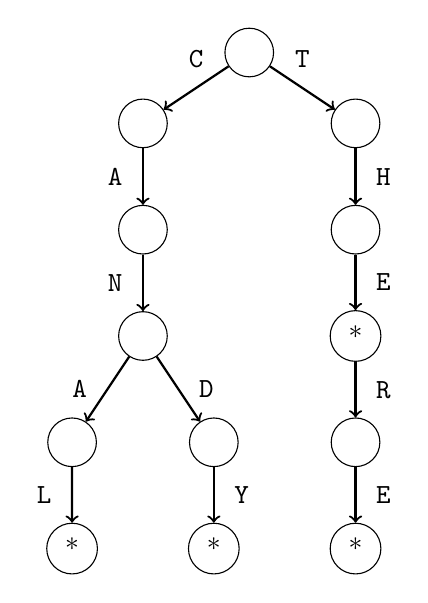
\begin{tikzpicture}[scale=0.9]
\node[draw, circle] (1) at (0,20) {$\phantom{1}$};
\node[draw, circle] (2) at (-1.5,19) {$\phantom{1}$};
\node[draw, circle] (3) at (1.5,19) {$\phantom{1}$};
\node[draw, circle] (4) at (-1.5,17.5) {$\phantom{1}$};
\node[draw, circle] (5) at (-1.5,16) {$\phantom{1}$};
\node[draw, circle] (6) at (-2.5,14.5) {$\phantom{1}$};
\node[draw, circle] (7) at (-0.5,14.5) {$\phantom{1}$};
\node[draw, circle] (8) at (-2.5,13) {*};
\node[draw, circle] (9) at (-0.5,13) {*};
\node[draw, circle] (10) at (1.5,17.5) {$\phantom{1}$};
\node[draw, circle] (11) at (1.5,16) {*};
\node[draw, circle] (12) at (1.5,14.5) {$\phantom{1}$};
\node[draw, circle] (13) at (1.5,13) {*};

\path[draw,thick,->] (1) -- node[font=\small,label=\texttt{C}] {} (2);
\path[draw,thick,->] (1) -- node[font=\small,label=\texttt{T}] {} (3);
\path[draw,thick,->] (2) -- node[font=\small,label=left:\texttt{A}] {} (4);
\path[draw,thick,->] (4) -- node[font=\small,label=left:\texttt{N}] {} (5);
\path[draw,thick,->] (5) -- node[font=\small,label=left:\texttt{A}] {} (6);
\path[draw,thick,->] (5) -- node[font=\small,label=right:\texttt{D}] {} (7);
\path[draw,thick,->] (6) -- node[font=\small,label=left:\texttt{L}] {}(8);
\path[draw,thick,->] (7) -- node[font=\small,label=right:\texttt{Y}] {} (9);
\path[draw,thick,->] (3) -- node[font=\small,label=right:\texttt{H}] {} (10);
\path[draw,thick,->] (10) -- node[font=\small,label=right:\texttt{E}] {} (11);
\path[draw,thick,->] (11) -- node[font=\small,label=right:\texttt{R}] {} (12);
\path[draw,thick,->] (12) -- node[font=\small,label=right:\texttt{E}] {} (13);
\end{tikzpicture}
\end{center}

このトライは、
$\{\texttt{CANAL},\texttt{CANDY},\texttt{THE},\texttt{THERE}\}$
を対応しています。
ノードにある文字*は、
集合の中の文字列がそのノードで終わることを示します。
このような情報がが必要なのは、
ある文字列が他の文字列の接頭辞である場合があるためです。
たとえば、上のトライでは\texttt{THE}は\texttt{THERE}のプレフィックスです。

根から始まるパスをたどればよいのでトライが長さ$n$の文字列を含むかどうかは$O(n)$時間で確認できます。
また、長さ$n$の文字列をトライに追加するにはパスを辿っていき必要ならトライに新しいノードを追加すればよいので$O(n)$で可能です。

トライを用いると与えられた文字列のうち、
その接頭辞が集合に属する最長のプレフィックスを求めることができます。
さらに各ノードに追加情報を格納することで、
集合に属してかつ、与えられた文字列を接頭辞として持つ文字列の数を計算することができます。

トライは配列に格納することができます。
\begin{lstlisting}
int trie[N][A];
\end{lstlisting}
ここで、$N$はノードの最大数(文字列の最大合計長)、
$A$はアルファ ベットの大きさです。
トライのノードはルートの番号が0になるように$0,1,2,\ldots$ と番号付けを行い、
$\texttt{trie}[s][c]$はノード$s$から文字$c$を使って移動したときの次のノードを示します。

\section{文字列のハッシュ化 - String hashing}

\index{ハッシュ - hashing}
\index{文字列のハッシュ化 - string hashing}

\key{文字列のハッシュ化 - String hashing}
は2つの文字列が等しいかどうかを効率的にチェックするためのテクニック\footnote{The technique
was popularized by the Karp–Rabin pattern matching
algorithm \cite{kar87}.}
です。
文字列ハッシュは文字単位ではなく文字列全体のハッシュ値を用います。

\subsubsection*{ハッシュ値の計算 - Calculating hash values}

\index{ハッシュ値 - hash value}
\index{多項式ハッシュ - polynomial hashing}

文字列の\key{ハッシュ値 - hash value}
は文字列全体の文字から算出される数値のことです。
決まったルールで算出を行うので2つの文字列が同じであればハッシュ値も同じになり、
ハッシュ値をもとに文字列を比較することができます。
通常、この実装方法は多項式ハッシュであり長さ$n$の文字列\texttt{s}のハッシュ値として

\[(\texttt{s}[0] A^{n-1} + \texttt{s}[1] A^{n-2} + \cdots + \texttt{s}[n-1] A^0) \bmod B  ,\]

と示され、ここで、
$s[0],s[1],\ldots,s[n-1]$
は\texttt{s}の各文字を示し、$A$と$B$はあらかじめ選択した定数となります。

例えば文字列\texttt{ALLEY}を考えます。
\begin{center}
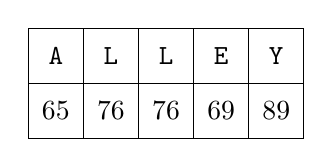
\begin{tikzpicture}[scale=0.7]
\draw (0,0) grid (5,2);

\node at (0.5, 1.5) {\texttt{A}};
\node at (1.5, 1.5) {\texttt{L}};
\node at (2.5, 1.5) {\texttt{L}};
\node at (3.5, 1.5) {\texttt{E}};
\node at (4.5, 1.5) {\texttt{Y}};

\node at (0.5, 0.5) {65};
\node at (1.5, 0.5) {76};
\node at (2.5, 0.5) {76};
\node at (3.5, 0.5) {69};
\node at (4.5, 0.5) {89};

\end{tikzpicture}
\end{center}

$A=3$、$B=97$とするとこのハッシュ値は
\[(65 \cdot 3^4 + 76 \cdot 3^3 + 76 \cdot 3^2 + 69 \cdot 3^1 + 89 \cdot 3^0) \bmod 97 = 52.\]

\subsubsection*{前処理 - Preprocessing}

多項式ハッシュを用いることで
文字列\texttt{s}の任意の部分文字列のハッシュ値を$O(n)$で求めて、
この前処理を行った後は$O(1)$時間で計算することができます。
このアイデアは $h[k]$ が接頭辞$\texttt{s}[0 \ldots k]$
のハッシュ値を含むような配列$h$を構築していることです。
配列の値は以下のように再帰的に計算することができます。

\[
\begin{array}{lcl}
\texttt{h}[0] & = & \texttt{s}[0] \\
\texttt{h}[k] & = & (\texttt{h}[k-1] A + \texttt{s}[k]) \bmod B \\
\end{array}
\]
さらに$\texttt{p}[k]=A^k \bmod B$となる配列$\texttt{p}$を構築します。
\[
\begin{array}{lcl}
\texttt{p}[0] & = & 1 \\
\texttt{p}[k] & = & (\texttt{p}[k-1] A) \bmod B. \\
\end{array}
\]
これらの配列の構築は$O(n)$で行えます。
この後に任意の部分文字列$\texttt{s}[a \ldots b]$のハッシュ値は
$a>0$である場合、以下の式を用いて$O(1)$で計算することができます。
\[(\texttt{h}[b]-\texttt{h}[a-1] \texttt{p}[b-a+1]) \bmod B\]
$a=0$の場合は単に\texttt{h}[b]となります。

\subsubsection*{ハッシュ値の利用 - Using hash values}

このような文字列のハッシュ値を使うと文字列を効率的に比較することができます。
ハッシュ値が等しければ、文字列はおそらく等しく(訳注: ハッシュの衝突の可能性がゼロとはいえないのでおそらくとなっています)、
ハッシュ値が異なれば、文字列は確実に異なります。

ハッシュ化の活用としてブルートフォースアルゴリズムを効率化できるケースがあります。
例えば文字列$s$とパターン$p$が与えられたとき$s$の中で$p$が出現する位置を見つけるというパターンマッチング問題を考えます。
ブルートフォースアルゴリズムは$p$が出現しそうな位置をすべて調べ、
文字列を1文字ずつ比較する手法ですが、このようなアルゴリズムの時間計算量は$O(n^2)$です。

これをハッシュ値を使用することでより効率的にすることができます。
ハッシュを用いると部分文字列のハッシュ値のみが比較されるため各比較は$O(1)$しかかりません。
この結果、時間計算量$O(n)$のアルゴリズムとなってとても良い時間計算量となります。

ハッシュと二分探索を組み合わせることで、
2つの文字列の辞書的順序を対数時間で求めることも可能できます。
2つの文字列の共通接頭辞の長さを二分探索で計算します。
こうして共通の接頭辞の長さがわかればあとは接頭辞の次の文字を($O(1)$で)調べればよいのです。

\subsubsection*{衝突と定数パラメータ - Collisions and parameters}

\index{衝突 - collision}

ハッシュ値を利用する際にはハッシュ値の\key{衝突 - collision}を考慮
しないとなりません。
ハッシュ値に依存するアルゴリズムは、もしハッシュ値の衝突が発生してしまうと、
2つの文字列が等しいと判定してしまいます。

一般的に存在する文字列の数はハッシュ値で表現できる数より大きいので、
衝突は常に起こりうる問題です。
しかし、定数$A$、$B$を上手く選べば衝突の確率は小さくできます。
通常の方法は、$10^9$ に近いランダムな定数を以下のように選ぶことです。

\[
\begin{array}{lcl}
A & = & 911382323 \\
B & = & 972663749 \\
\end{array}
\]

この定数を使うと、ハッシュ値を計算するときに、
$AB$と$BB$の積が\texttt{long long}に収まるので、
\texttt{long long}型が使えます。
さて、ハッシュ値は$10^9$くらいあれば十分なのでしょうか?

次の3つのシナリオを考えてみましょう。

\textit{Scenario 1:} 文字列$x$と$y$を比較する。
衝突の確率は、全てのハッシュ値が等確率であると仮定すると$1/B$となる。

\textit{Scenario 2:} 文字列$x$ を複数の文字列
$y_1,y_2,\ldots,y_n$と比較する。
この時の1つ以上の衝突の確率は次の通り。

\[1-(1-\frac{1}{B})^n.\]

\textit{Scenario 3:} 複数の文字列$x_1,x_2,\ldots,x_n$
を全て互いに比較したとする。
この時の1つ以上の衝突の確率は次の通り。
\[ 1 - \frac{B \cdot (B-1) \cdot (B-2) \cdots (B-n+1)}{B^n}.\]

$n=10^6$として$b$を変化させた衝突確率を以下に示します。

\begin{center}
\begin{tabular}{rrrr}
定数 $B$ & scenario 1 & scenario 2 & scenario 3 \\
\hline
$10^3$ & $0.001000$ & $1.000000$ & $1.000000$ \\
$10^6$ & $0.000001$ & $0.632121$ & $1.000000$ \\
$10^9$ & $0.000000$ & $0.001000$ & $1.000000$ \\
$10^{12}$ & $0.000000$ & $0.000000$ & $0.393469$ \\
$10^{15}$ & $0.000000$ & $0.000000$ & $0.000500$ \\
$10^{18}$ & $0.000000$ & $0.000000$ & $0.000001$ \\
\end{tabular}
\end{center}

表から、シナリオ1では、$B \approx 10^9$ のとき、
衝突の確率は無視できる程度です。
シナリオ2では、衝突の可能性はあるが、その確率はまだかなり小さいです。
しかし、シナリオ3では状況は大きく異なり、$B \approx 10^9$のとき、
かなりの確率で衝突が起こります。

\index{誕生日のパラドックス - birthday paradox}

シナリオ3の現象は、\key{誕生日のパラドックス -birthday paradox}
として知られている問題です。
$n$人いれば、$n$がかなり小さくても同じ誕生日の人がいる確率は大きくなります。
これがハッシュでも同じことが言えます。

そこで、異なるパラメータを用いて\emph{複数}のハッシュ値を計算することで、
衝突の確率を小さくすることができます。
この場合にすべてのハッシュ値で同時に衝突が発生することは考えにくくなります。
例えばパラメータ$B \approx 10^9$のハッシュ値2個は、
パラメータ$B \approx 10^18$のハッシュ値1個に相当するため衝突の可能性を格段に下げることができます。

定数として $B=2^{32}$ と $B=2^{64}$を選択する人もいます。
これは、$2^{32}$ や $2^{64}$でのmodをとると32bit長や64bit長の
型で計算できるために良いように思えます。
しかし、これは良い選択ではありません。$2^x$の形の定数は
衝突を発生させる入力を構成することが可能だからです\cite{pac13}。

\section{Z-アルゴリズム - Z-algorithm}

\index{Z-アルゴリズム - Z-algorithm}
\index{Z配列 - Z-array}

長さ$n$の文字列$s$の\key{Z配列 - Z-array}である$z$は、
$k=0,1,\ldots,n-1$に対して、
$k$の位置から始まる$s$の最長の部分文字列の長さと$s$の接頭辞を含みます。
したがって、$\texttt{z}[k]=p$は
$\texttt{s}[0 \ldots p-1]$が$\texttt{s}[k \ldots k+p-1]$に
等しいことを意味します。
文字列処理の問題の多くは、Z配列を使うと効果的に解くことができます。

\texttt{ACBACDACBACBACDA} のZ配列の例を示します。

\begin{center}
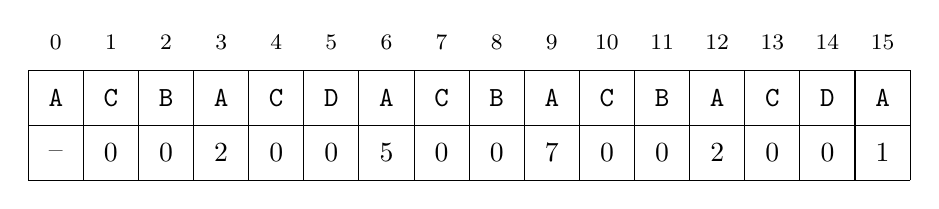
\begin{tikzpicture}[scale=0.7]
\draw (0,0) grid (16,2);

\node at (0.5, 1.5) {\texttt{A}};
\node at (1.5, 1.5) {\texttt{C}};
\node at (2.5, 1.5) {\texttt{B}};
\node at (3.5, 1.5) {\texttt{A}};
\node at (4.5, 1.5) {\texttt{C}};
\node at (5.5, 1.5) {\texttt{D}};
\node at (6.5, 1.5) {\texttt{A}};
\node at (7.5, 1.5) {\texttt{C}};
\node at (8.5, 1.5) {\texttt{B}};
\node at (9.5, 1.5) {\texttt{A}};
\node at (10.5, 1.5) {\texttt{C}};
\node at (11.5, 1.5) {\texttt{B}};
\node at (12.5, 1.5) {\texttt{A}};
\node at (13.5, 1.5) {\texttt{C}};
\node at (14.5, 1.5) {\texttt{D}};
\node at (15.5, 1.5) {\texttt{A}};

\node at (0.5, 0.5) {--};
\node at (1.5, 0.5) {0};
\node at (2.5, 0.5) {0};
\node at (3.5, 0.5) {2};
\node at (4.5, 0.5) {0};
\node at (5.5, 0.5) {0};
\node at (6.5, 0.5) {5};
\node at (7.5, 0.5) {0};
\node at (8.5, 0.5) {0};
\node at (9.5, 0.5) {7};
\node at (10.5, 0.5) {0};
\node at (11.5, 0.5) {0};
\node at (12.5, 0.5) {2};
\node at (13.5, 0.5) {0};
\node at (14.5, 0.5) {0};
\node at (15.5, 0.5) {1};

\footnotesize
\node at (0.5, 2.5) {0};
\node at (1.5, 2.5) {1};
\node at (2.5, 2.5) {2};
\node at (3.5, 2.5) {3};
\node at (4.5, 2.5) {4};
\node at (5.5, 2.5) {5};
\node at (6.5, 2.5) {6};
\node at (7.5, 2.5) {7};
\node at (8.5, 2.5) {8};
\node at (9.5, 2.5) {9};
\node at (10.5, 2.5) {10};
\node at (11.5, 2.5) {11};
\node at (12.5, 2.5) {12};
\node at (13.5, 2.5) {13};
\node at (14.5, 2.5) {14};
\node at (15.5, 2.5) {15};

\end{tikzpicture}
\end{center}

このケースでは$\texttt{z}[6]=5$となります。
部分文字列\texttt{ACBAC}は長さ5の\texttt{s}のプレフィックスですが、
部分文字列\texttt{ACBACB}という長さ6の\texttt{s}のプレフィックスではないからです。

\subsubsection*{Zアルゴリズムの説明 - Algorithm description}

これを求めるアルゴリズムを紹介していきます。
\key{Zアルゴリズム - Z-algorithm}\footnote{The Z-algorithm
was presented in \cite{gus97} as the simplest known
method for linear-time pattern matching, and the original idea
was attributed to \cite{mai84}.}
と呼ばれる、Z配列を $O(n)$ 時間で効率的に構成するアルゴリズムがあります。
このアルゴリズムは、Z配列に既に格納されている情報を利用し、
また、文字列を一文字ずつ比較することでZ配列の値を左から右へと計算していきます。

Z配列の値を効率的に計算するために、
アルゴリズムは$\texttt{s}[x \ldots y]$が$s$の接頭辞で、
$y$ができるだけ大きくなるような区間$[x, y]$を維持します。
$\texttt{s}[0 \ldots y-x]$と$\texttt{s}[x \ldots y]$は等しいことが分かっているので、
位置$x+1,x+2,\ldots,y$のZ値を計算するときにこの情報を利用できます。

各位置$k$で$\texttt{z}[k-x]$の値を確認します。
$k+\texttt{z}[k-x]<y$ならば、$\texttt{z}[k]=\texttt{z}[k-x]$です。
しかし、$k+\texttt{z}[k-x] \ge y$の場合は
$\texttt{s}[0 \ldots y-k]$ は
$\texttt{s}[k \ldots y]$ と等しく、
$\texttt{z}[k]$の値を決定するためには、部分文字列の文字列を比較する必要があります。
このアルゴリズムは$O(n)$で動作します。なぜなら、比較が
$y-k+1$ と $y+1$ で行われるためです。

例えば、次のようなZ配列を考えます。

\begin{center}
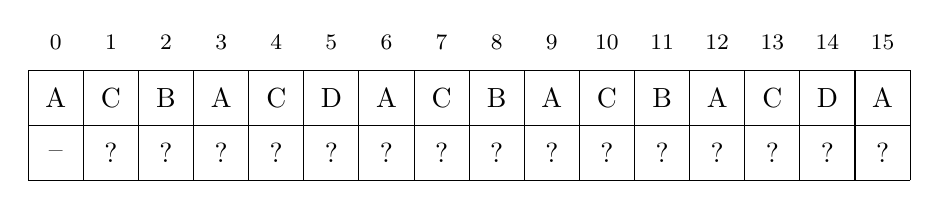
\begin{tikzpicture}[scale=0.7]
\draw (0,0) grid (16,2);

\node at (0.5, 1.5) {A};
\node at (1.5, 1.5) {C};
\node at (2.5, 1.5) {B};
\node at (3.5, 1.5) {A};
\node at (4.5, 1.5) {C};
\node at (5.5, 1.5) {D};
\node at (6.5, 1.5) {A};
\node at (7.5, 1.5) {C};
\node at (8.5, 1.5) {B};
\node at (9.5, 1.5) {A};
\node at (10.5, 1.5) {C};
\node at (11.5, 1.5) {B};
\node at (12.5, 1.5) {A};
\node at (13.5, 1.5) {C};
\node at (14.5, 1.5) {D};
\node at (15.5, 1.5) {A};

\node at (0.5, 0.5) {--};
\node at (1.5, 0.5) {?};
\node at (2.5, 0.5) {?};
\node at (3.5, 0.5) {?};
\node at (4.5, 0.5) {?};
\node at (5.5, 0.5) {?};
\node at (6.5, 0.5) {?};
\node at (7.5, 0.5) {?};
\node at (8.5, 0.5) {?};
\node at (9.5, 0.5) {?};
\node at (10.5, 0.5) {?};
\node at (11.5, 0.5) {?};
\node at (12.5, 0.5) {?};
\node at (13.5, 0.5) {?};
\node at (14.5, 0.5) {?};
\node at (15.5, 0.5) {?};

\footnotesize
\node at (0.5, 2.5) {0};
\node at (1.5, 2.5) {1};
\node at (2.5, 2.5) {2};
\node at (3.5, 2.5) {3};
\node at (4.5, 2.5) {4};
\node at (5.5, 2.5) {5};
\node at (6.5, 2.5) {6};
\node at (7.5, 2.5) {7};
\node at (8.5, 2.5) {8};
\node at (9.5, 2.5) {9};
\node at (10.5, 2.5) {10};
\node at (11.5, 2.5) {11};
\node at (12.5, 2.5) {12};
\node at (13.5, 2.5) {13};
\node at (14.5, 2.5) {14};
\node at (15.5, 2.5) {15};

\end{tikzpicture}
\end{center}

$\texttt{z}[6]=5$を計算し$[x,y]$ のレンジは $[6,10]$となります。

\begin{center}
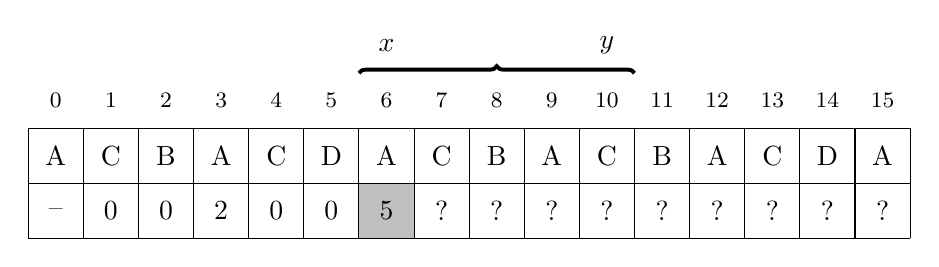
\begin{tikzpicture}[scale=0.7]
\fill[color=lightgray] (6,0) rectangle (7,1);
\draw (0,0) grid (16,2);

\node at (0.5, 1.5) {A};
\node at (1.5, 1.5) {C};
\node at (2.5, 1.5) {B};
\node at (3.5, 1.5) {A};
\node at (4.5, 1.5) {C};
\node at (5.5, 1.5) {D};
\node at (6.5, 1.5) {A};
\node at (7.5, 1.5) {C};
\node at (8.5, 1.5) {B};
\node at (9.5, 1.5) {A};
\node at (10.5, 1.5) {C};
\node at (11.5, 1.5) {B};
\node at (12.5, 1.5) {A};
\node at (13.5, 1.5) {C};
\node at (14.5, 1.5) {D};
\node at (15.5, 1.5) {A};

\node at (0.5, 0.5) {--};
\node at (1.5, 0.5) {0};
\node at (2.5, 0.5) {0};
\node at (3.5, 0.5) {2};
\node at (4.5, 0.5) {0};
\node at (5.5, 0.5) {0};
\node at (6.5, 0.5) {5};
\node at (7.5, 0.5) {?};
\node at (8.5, 0.5) {?};
\node at (9.5, 0.5) {?};
\node at (10.5, 0.5) {?};
\node at (11.5, 0.5) {?};
\node at (12.5, 0.5) {?};
\node at (13.5, 0.5) {?};
\node at (14.5, 0.5) {?};
\node at (15.5, 0.5) {?};

\draw [decoration={brace}, decorate, line width=0.5mm] (6,3.00) -- (11,3.00);

\node at (6.5,3.50) {$x$};
\node at (10.5,3.50) {$y$};


\footnotesize
\node at (0.5, 2.5) {0};
\node at (1.5, 2.5) {1};
\node at (2.5, 2.5) {2};
\node at (3.5, 2.5) {3};
\node at (4.5, 2.5) {4};
\node at (5.5, 2.5) {5};
\node at (6.5, 2.5) {6};
\node at (7.5, 2.5) {7};
\node at (8.5, 2.5) {8};
\node at (9.5, 2.5) {9};
\node at (10.5, 2.5) {10};
\node at (11.5, 2.5) {11};
\node at (12.5, 2.5) {12};
\node at (13.5, 2.5) {13};
\node at (14.5, 2.5) {14};
\node at (15.5, 2.5) {15};

\end{tikzpicture}
\end{center}

これで
$\texttt{s}[0 \ldots 4]$と
$\texttt{s}[6 \ldots 10]$
が等しいことがわかったので、以降のZ配列の値を効率的に計算できるようになります。
まず、$\texttt{z}[1] = \texttt{z}[2] = 0$なので$\texttt{z}[7] = \texttt{z}[8] = 0$もすぐにわかります。

\begin{center}
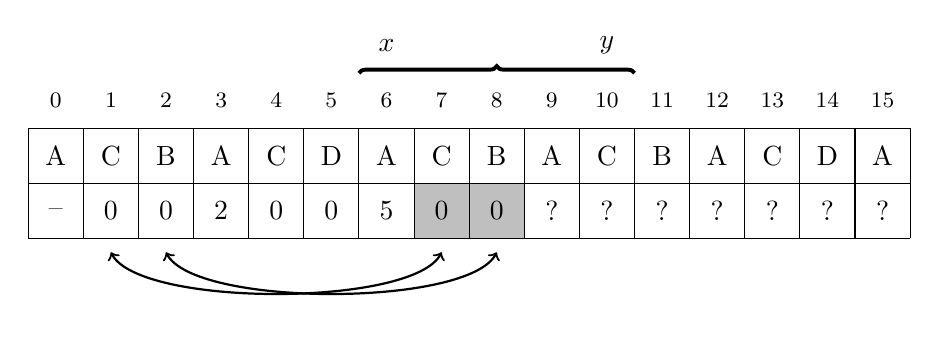
\begin{tikzpicture}[scale=0.7]
\fill[color=lightgray] (7,0) rectangle (9,1);
\draw (0,0) grid (16,2);

\node at (0.5, 1.5) {A};
\node at (1.5, 1.5) {C};
\node at (2.5, 1.5) {B};
\node at (3.5, 1.5) {A};
\node at (4.5, 1.5) {C};
\node at (5.5, 1.5) {D};
\node at (6.5, 1.5) {A};
\node at (7.5, 1.5) {C};
\node at (8.5, 1.5) {B};
\node at (9.5, 1.5) {A};
\node at (10.5, 1.5) {C};
\node at (11.5, 1.5) {B};
\node at (12.5, 1.5) {A};
\node at (13.5, 1.5) {C};
\node at (14.5, 1.5) {D};
\node at (15.5, 1.5) {A};

\node at (0.5, 0.5) {--};
\node at (1.5, 0.5) {0};
\node at (2.5, 0.5) {0};
\node at (3.5, 0.5) {2};
\node at (4.5, 0.5) {0};
\node at (5.5, 0.5) {0};
\node at (6.5, 0.5) {5};
\node at (7.5, 0.5) {0};
\node at (8.5, 0.5) {0};
\node at (9.5, 0.5) {?};
\node at (10.5, 0.5) {?};
\node at (11.5, 0.5) {?};
\node at (12.5, 0.5) {?};
\node at (13.5, 0.5) {?};
\node at (14.5, 0.5) {?};
\node at (15.5, 0.5) {?};


\draw [decoration={brace}, decorate, line width=0.5mm] (6,3.00) -- (11,3.00);

\node at (6.5,3.50) {$x$};
\node at (10.5,3.50) {$y$};


\footnotesize
\node at (0.5, 2.5) {0};
\node at (1.5, 2.5) {1};
\node at (2.5, 2.5) {2};
\node at (3.5, 2.5) {3};
\node at (4.5, 2.5) {4};
\node at (5.5, 2.5) {5};
\node at (6.5, 2.5) {6};
\node at (7.5, 2.5) {7};
\node at (8.5, 2.5) {8};
\node at (9.5, 2.5) {9};
\node at (10.5, 2.5) {10};
\node at (11.5, 2.5) {11};
\node at (12.5, 2.5) {12};
\node at (13.5, 2.5) {13};
\node at (14.5, 2.5) {14};
\node at (15.5, 2.5) {15};


\draw[thick,<->] (7.5,-0.25) .. controls (7,-1.25) and (2,-1.25) .. (1.5,-0.25);
\draw[thick,<->] (8.5,-0.25) .. controls (8,-1.25) and (3,-1.25) .. (2.5,-0.25);
\end{tikzpicture}
\end{center}

ここで$\texttt{z}[3]=2$から$\texttt{z}[9] \ge 2$がわかります。

\begin{center}
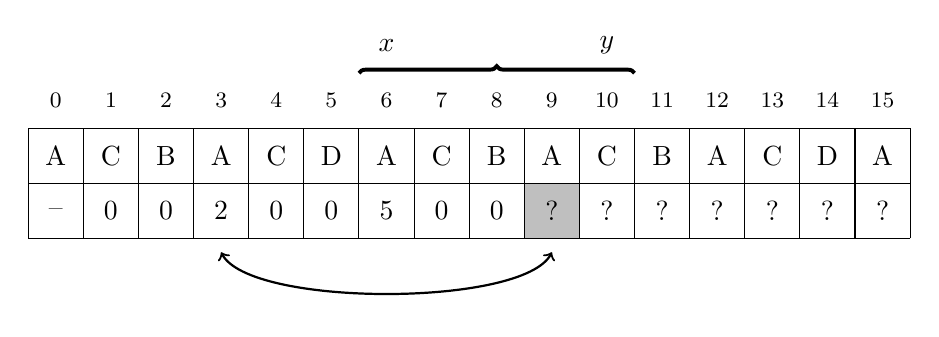
\begin{tikzpicture}[scale=0.7]
\fill[color=lightgray] (9,0) rectangle (10,1);
\draw (0,0) grid (16,2);

\node at (0.5, 1.5) {A};
\node at (1.5, 1.5) {C};
\node at (2.5, 1.5) {B};
\node at (3.5, 1.5) {A};
\node at (4.5, 1.5) {C};
\node at (5.5, 1.5) {D};
\node at (6.5, 1.5) {A};
\node at (7.5, 1.5) {C};
\node at (8.5, 1.5) {B};
\node at (9.5, 1.5) {A};
\node at (10.5, 1.5) {C};
\node at (11.5, 1.5) {B};
\node at (12.5, 1.5) {A};
\node at (13.5, 1.5) {C};
\node at (14.5, 1.5) {D};
\node at (15.5, 1.5) {A};

\node at (0.5, 0.5) {--};
\node at (1.5, 0.5) {0};
\node at (2.5, 0.5) {0};
\node at (3.5, 0.5) {2};
\node at (4.5, 0.5) {0};
\node at (5.5, 0.5) {0};
\node at (6.5, 0.5) {5};
\node at (7.5, 0.5) {0};
\node at (8.5, 0.5) {0};
\node at (9.5, 0.5) {?};
\node at (10.5, 0.5) {?};
\node at (11.5, 0.5) {?};
\node at (12.5, 0.5) {?};
\node at (13.5, 0.5) {?};
\node at (14.5, 0.5) {?};
\node at (15.5, 0.5) {?};

\draw [decoration={brace}, decorate, line width=0.5mm] (6,3.00) -- (11,3.00);

\node at (6.5,3.50) {$x$};
\node at (10.5,3.50) {$y$};


\footnotesize
\node at (0.5, 2.5) {0};
\node at (1.5, 2.5) {1};
\node at (2.5, 2.5) {2};
\node at (3.5, 2.5) {3};
\node at (4.5, 2.5) {4};
\node at (5.5, 2.5) {5};
\node at (6.5, 2.5) {6};
\node at (7.5, 2.5) {7};
\node at (8.5, 2.5) {8};
\node at (9.5, 2.5) {9};
\node at (10.5, 2.5) {10};
\node at (11.5, 2.5) {11};
\node at (12.5, 2.5) {12};
\node at (13.5, 2.5) {13};
\node at (14.5, 2.5) {14};
\node at (15.5, 2.5) {15};

\draw[thick,<->] (9.5,-0.25) .. controls (9,-1.25) and (4,-1.25) .. (3.5,-0.25);
\end{tikzpicture}
\end{center}

10以降の文字列については情報がないので文字ごとに部分文字列を比較します。

\begin{center}
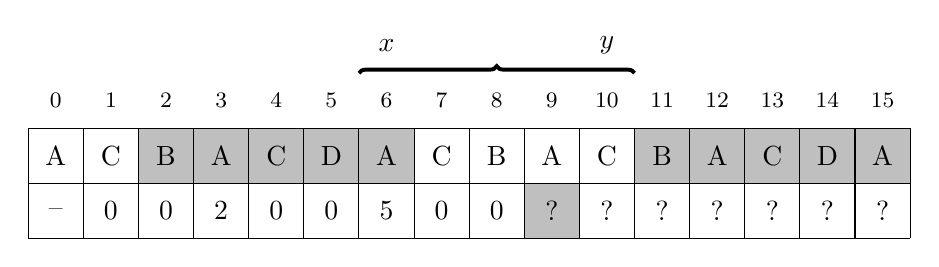
\begin{tikzpicture}[scale=0.7]
\fill[color=lightgray] (9,0) rectangle (10,1);
\fill[color=lightgray] (2,1) rectangle (7,2);
\fill[color=lightgray] (11,1) rectangle (16,2);


\draw (0,0) grid (16,2);

\node at (0.5, 1.5) {A};
\node at (1.5, 1.5) {C};
\node at (2.5, 1.5) {B};
\node at (3.5, 1.5) {A};
\node at (4.5, 1.5) {C};
\node at (5.5, 1.5) {D};
\node at (6.5, 1.5) {A};
\node at (7.5, 1.5) {C};
\node at (8.5, 1.5) {B};
\node at (9.5, 1.5) {A};
\node at (10.5, 1.5) {C};
\node at (11.5, 1.5) {B};
\node at (12.5, 1.5) {A};
\node at (13.5, 1.5) {C};
\node at (14.5, 1.5) {D};
\node at (15.5, 1.5) {A};

\node at (0.5, 0.5) {--};
\node at (1.5, 0.5) {0};
\node at (2.5, 0.5) {0};
\node at (3.5, 0.5) {2};
\node at (4.5, 0.5) {0};
\node at (5.5, 0.5) {0};
\node at (6.5, 0.5) {5};
\node at (7.5, 0.5) {0};
\node at (8.5, 0.5) {0};
\node at (9.5, 0.5) {?};
\node at (10.5, 0.5) {?};
\node at (11.5, 0.5) {?};
\node at (12.5, 0.5) {?};
\node at (13.5, 0.5) {?};
\node at (14.5, 0.5) {?};
\node at (15.5, 0.5) {?};

\draw [decoration={brace}, decorate, line width=0.5mm] (6,3.00) -- (11,3.00);

\node at (6.5,3.50) {$x$};
\node at (10.5,3.50) {$y$};


\footnotesize
\node at (0.5, 2.5) {0};
\node at (1.5, 2.5) {1};
\node at (2.5, 2.5) {2};
\node at (3.5, 2.5) {3};
\node at (4.5, 2.5) {4};
\node at (5.5, 2.5) {5};
\node at (6.5, 2.5) {6};
\node at (7.5, 2.5) {7};
\node at (8.5, 2.5) {8};
\node at (9.5, 2.5) {9};
\node at (10.5, 2.5) {10};
\node at (11.5, 2.5) {11};
\node at (12.5, 2.5) {12};
\node at (13.5, 2.5) {13};
\node at (14.5, 2.5) {14};
\node at (15.5, 2.5) {15};

%\draw[thick,<->] (11.5,-0.25) .. controls (11,-1.25) and (3,-1.25) .. (2.5,-0.25);
\end{tikzpicture}
\end{center}

$\texttt{z}[9]=7$となったので新しい$[x,y]$は$[9,15]$となります。

\begin{center}
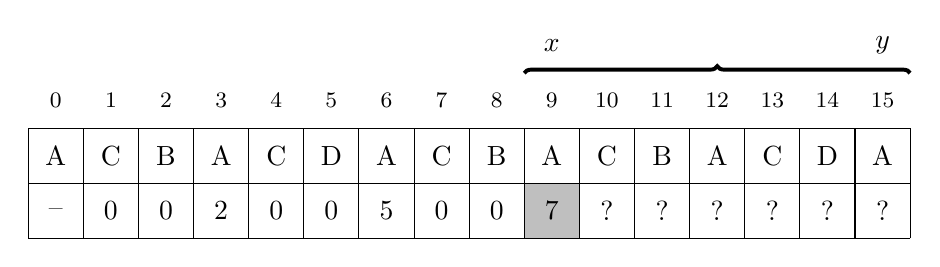
\begin{tikzpicture}[scale=0.7]
\fill[color=lightgray] (9,0) rectangle (10,1);
\draw (0,0) grid (16,2);

\node at (0.5, 1.5) {A};
\node at (1.5, 1.5) {C};
\node at (2.5, 1.5) {B};
\node at (3.5, 1.5) {A};
\node at (4.5, 1.5) {C};
\node at (5.5, 1.5) {D};
\node at (6.5, 1.5) {A};
\node at (7.5, 1.5) {C};
\node at (8.5, 1.5) {B};
\node at (9.5, 1.5) {A};
\node at (10.5, 1.5) {C};
\node at (11.5, 1.5) {B};
\node at (12.5, 1.5) {A};
\node at (13.5, 1.5) {C};
\node at (14.5, 1.5) {D};
\node at (15.5, 1.5) {A};

\node at (0.5, 0.5) {--};
\node at (1.5, 0.5) {0};
\node at (2.5, 0.5) {0};
\node at (3.5, 0.5) {2};
\node at (4.5, 0.5) {0};
\node at (5.5, 0.5) {0};
\node at (6.5, 0.5) {5};
\node at (7.5, 0.5) {0};
\node at (8.5, 0.5) {0};
\node at (9.5, 0.5) {7};
\node at (10.5, 0.5) {?};
\node at (11.5, 0.5) {?};
\node at (12.5, 0.5) {?};
\node at (13.5, 0.5) {?};
\node at (14.5, 0.5) {?};
\node at (15.5, 0.5) {?};

\draw [decoration={brace}, decorate, line width=0.5mm] (9,3.00) -- (16,3.00);

\node at (9.5,3.50) {$x$};
\node at (15.5,3.50) {$y$};


\footnotesize
\node at (0.5, 2.5) {0};
\node at (1.5, 2.5) {1};
\node at (2.5, 2.5) {2};
\node at (3.5, 2.5) {3};
\node at (4.5, 2.5) {4};
\node at (5.5, 2.5) {5};
\node at (6.5, 2.5) {6};
\node at (7.5, 2.5) {7};
\node at (8.5, 2.5) {8};
\node at (9.5, 2.5) {9};
\node at (10.5, 2.5) {10};
\node at (11.5, 2.5) {11};
\node at (12.5, 2.5) {12};
\node at (13.5, 2.5) {13};
\node at (14.5, 2.5) {14};
\node at (15.5, 2.5) {15};

% \draw[thick,<->] (9.5,-0.25) .. controls (9,-1.25) and (4,-1.25) .. (3.5,-0.25);
\end{tikzpicture}
\end{center}

あとは、Z配列の値を使って他のZ配列の文字列を決めることができます。

\begin{center}
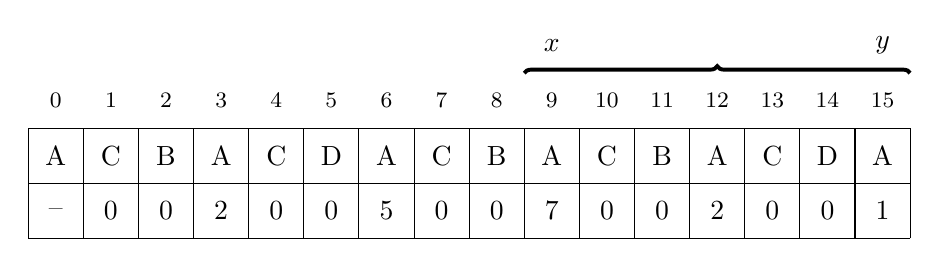
\begin{tikzpicture}[scale=0.7]
\draw (0,0) grid (16,2);

\node at (0.5, 1.5) {A};
\node at (1.5, 1.5) {C};
\node at (2.5, 1.5) {B};
\node at (3.5, 1.5) {A};
\node at (4.5, 1.5) {C};
\node at (5.5, 1.5) {D};
\node at (6.5, 1.5) {A};
\node at (7.5, 1.5) {C};
\node at (8.5, 1.5) {B};
\node at (9.5, 1.5) {A};
\node at (10.5, 1.5) {C};
\node at (11.5, 1.5) {B};
\node at (12.5, 1.5) {A};
\node at (13.5, 1.5) {C};
\node at (14.5, 1.5) {D};
\node at (15.5, 1.5) {A};

\node at (0.5, 0.5) {--};
\node at (1.5, 0.5) {0};
\node at (2.5, 0.5) {0};
\node at (3.5, 0.5) {2};
\node at (4.5, 0.5) {0};
\node at (5.5, 0.5) {0};
\node at (6.5, 0.5) {5};
\node at (7.5, 0.5) {0};
\node at (8.5, 0.5) {0};
\node at (9.5, 0.5) {7};
\node at (10.5, 0.5) {0};
\node at (11.5, 0.5) {0};
\node at (12.5, 0.5) {2};
\node at (13.5, 0.5) {0};
\node at (14.5, 0.5) {0};
\node at (15.5, 0.5) {1};

\draw [decoration={brace}, decorate, line width=0.5mm] (9,3.00) -- (16,3.00);

\node at (9.5,3.50) {$x$};
\node at (15.5,3.50) {$y$};


\footnotesize
\node at (0.5, 2.5) {0};
\node at (1.5, 2.5) {1};
\node at (2.5, 2.5) {2};
\node at (3.5, 2.5) {3};
\node at (4.5, 2.5) {4};
\node at (5.5, 2.5) {5};
\node at (6.5, 2.5) {6};
\node at (7.5, 2.5) {7};
\node at (8.5, 2.5) {8};
\node at (9.5, 2.5) {9};
\node at (10.5, 2.5) {10};
\node at (11.5, 2.5) {11};
\node at (12.5, 2.5) {12};
\node at (13.5, 2.5) {13};
\node at (14.5, 2.5) {14};
\node at (15.5, 2.5) {15};

\end{tikzpicture}
\end{center}

\subsubsection{Z配列の利用シーン - Using the Z-array}

文字列ハッシュとZ-アルゴリズムのどちらを使うかは、
好みの問題であるケースが多いです。
ハッシュとは異なり、Z-アルゴリズムには衝突の危険性がありません。
一方、Z-アルゴリズムは実装が難しく、
また、いくつかの問題はハッシュを使うことでしか解決できません。

試しに文字列$s$の中にあるパターン$p$の出現を見つけるというパターンマッチングの問題を考えます。
すでに文字列ハッシュを使って解決しましたが、Z-アルゴリズムでの解決方法があります。

Zアルゴリズムで文字列処理するためには、
特殊文字で区切られた複数の文字列からなる1つの文字列を構成するのが一般的な考え方です。
この問題では、pとsの文字列中に出現しない特殊文字\texttt{\#}で区切った
文字列$p$\texttt{\#}$s$を構築します。
$p$\texttt{\#}$s$のZ配列は、$s$の中で$p$が出現する位置を示すことになり、
その位置は$p$の長さを含んでいるためです。

例えば、$s=$\texttt{HATTIVATTI} で $p=$\texttt{ATT}としましょう。

\begin{center}
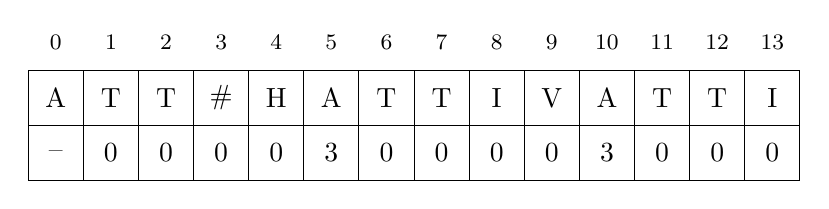
\begin{tikzpicture}[scale=0.7]
\draw (0,0) grid (14,2);

\node at (0.5, 1.5) {A};
\node at (1.5, 1.5) {T};
\node at (2.5, 1.5) {T};
\node at (3.5, 1.5) {\#};
\node at (4.5, 1.5) {H};
\node at (5.5, 1.5) {A};
\node at (6.5, 1.5) {T};
\node at (7.5, 1.5) {T};
\node at (8.5, 1.5) {I};
\node at (9.5, 1.5) {V};
\node at (10.5, 1.5) {A};
\node at (11.5, 1.5) {T};
\node at (12.5, 1.5) {T};
\node at (13.5, 1.5) {I};

\node at (0.5, 0.5) {--};
\node at (1.5, 0.5) {0};
\node at (2.5, 0.5) {0};
\node at (3.5, 0.5) {0};
\node at (4.5, 0.5) {0};
\node at (5.5, 0.5) {3};
\node at (6.5, 0.5) {0};
\node at (7.5, 0.5) {0};
\node at (8.5, 0.5) {0};
\node at (9.5, 0.5) {0};
\node at (10.5, 0.5) {3};
\node at (11.5, 0.5) {0};
\node at (12.5, 0.5) {0};
\node at (13.5, 0.5) {0};

\footnotesize
\node at (0.5, 2.5) {0};
\node at (1.5, 2.5) {1};
\node at (2.5, 2.5) {2};
\node at (3.5, 2.5) {3};
\node at (4.5, 2.5) {4};
\node at (5.5, 2.5) {5};
\node at (6.5, 2.5) {6};
\node at (7.5, 2.5) {7};
\node at (8.5, 2.5) {8};
\node at (9.5, 2.5) {9};
\node at (10.5, 2.5) {10};
\node at (11.5, 2.5) {11};
\node at (12.5, 2.5) {12};
\node at (13.5, 2.5) {13};
\end{tikzpicture}
\end{center}

5,10には長さ3が含まれているので、\texttt{ATT}が
\texttt{HATTIVATTI}のこの位置で発生していることがわかります。

Z配列の計算には線形時間がかかるため、この計算は線形で実行することができます。

\subsubsection{実装 - Implementation}

ここでは、Z配列を返すZアルゴリズムの実装を示します。

\begin{lstlisting}
vector<int> z(string s) {
    int n = s.size();
    vector<int> z(n);
    int x = 0, y = 0;
    for (int i = 1; i < n; i++) {
        z[i] = max(0,min(z[i-x],y-i+1));
        while (i+z[i] < n && s[z[i]] == s[i+z[i]]) {
            x = i; y = i+z[i]; z[i]++;
        }
    }
    return z;
}
\end{lstlisting}
